% =====================================================================
% Slides do Seminário 2 (12 min + 5 min de arguição)
% Compilar no Overleaf com pdfLaTeX (arquivo principal: slides.tex)
% Números e tabelas vêm de tabelas/*.tex (gerados pelo código).
% 11 slides principais; os slides de apoio (após "Obrigado") são para a arguição.
% =====================================================================
\documentclass[aspectratio=169,11pt]{beamer}

\usepackage[utf8]{inputenc}
\usepackage[T1]{fontenc}
\usepackage[brazil]{babel}
\usepackage{lmodern}
\usepackage{amsmath,amssymb}
\usepackage{booktabs}
\usepackage{array}
\usepackage{graphicx}
\usepackage{appendixnumberbeamer}

\graphicspath{{figuras/}}
% Gerado por gera_tabelas_latex.py -- não editar à mão
\newcommand{\lambdaCentral}{0{,}435}
\newcommand{\lambdaCalibrado}{0{,}435}
\newcommand{\lambdaGargalo}{0{,}43}
\newcommand{\lambdaMinLinha}{0{,}22}
\newcommand{\lambdaMaxLinha}{0{,}73}
\newcommand{\Zotimo}{276.041{,}95}
\newcommand{\custoTotal}{264.416{,}95}
\newcommand{\esperaPash}{465}
\newcommand{\esperaMin}{0{,}32}
\newcommand{\demandaTotal}{86.310}
\newcommand{\viagensTotal}{712}
\newcommand{\viagensGTFS}{664}
\newcommand{\variacaoViagens}{7{,}2}
\newcommand{\custoGTFS}{242.902{,}32}
\newcommand{\variacaoCusto}{8{,}9}
\newcommand{\esperaMinGTFS}{35{,}0}
\newcommand{\ZGTFS}{1.500.427}
\newcommand{\perdidosGTFS}{4.245}
\newcommand{\pctPerdidosGTFS}{4{,}92}
\newcommand{\perdidosOtimo}{392}
\newcommand{\pctPerdidosOtimo}{0{,}45}
\newcommand{\custoPerdaGTFS}{242.902}
\newcommand{\custoPerdaOtimo}{262.994}
\newcommand{\embViagemCentral}{130{,}0}
\newcommand{\embViagemUm}{171{,}2}
\newcommand{\esperaLambdaZero}{0{,}05}
\newcommand{\esperaLambdaUm}{8{,}36}
\newcommand{\frotaNecZero}{79}
\newcommand{\frotaNecUm}{102}
\newcommand{\frotaNecCentral}{99}
\newcommand{\precoLambdaUm}{13.255}
\newcommand{\frotaMax}{97}
\newcommand{\frotaMOVE}{457}
\newcommand{\capCorredor}{64}
\newcommand{\esperaFnoventa}{1{,}59}
\newcommand{\esperaMaisDezArt}{0{,}16}
\newcommand{\esperaPadron}{0{,}16}
\newcommand{\custoPadron}{256.980}
\newcommand{\custoMaisDezArt}{265.095}
\newcommand{\viagensPadron}{107}
\newcommand{\equilibrioPadron}{899}
\newcommand{\equilibrioMaisDezArt}{510}
\newcommand{\equilibrioPadronIgual}{340}
\newcommand{\viagensPadronIgual}{9}
\newcommand{\equilibrioMaisDezArtUm}{6.991}
\newcommand{\esperaBase}{0{,}32}
\newcommand{\custoBase}{264.417}
\newcommand{\esperaBaseUm}{8{,}36}
\newcommand{\esperaCorredorUm}{8{,}23}
\newcommand{\esperaMaisDezArtUm}{6{,}89}
\newcommand{\Zrelax}{257.280{,}40}
\newcommand{\gapInt}{6{,}80}
\newcommand{\gapFinal}{0{,}0031}
\newcommand{\cortesGomory}{26}
\newcommand{\cortesMIR}{64}
\newcommand{\nosExplorados}{1}
\newcommand{\iteracoesSimplex}{101}
\newcommand{\tempoSolucao}{0{,}11}
\newcommand{\presolveLinhas}{138}
\newcommand{\presolveColunas}{204}
\newcommand{\horaPrecoMax}{7h}
\newcommand{\precoSombraMax}{6.042{,}40}
\newcommand{\deltaPLIMMax}{2.971{,}26}
\newcommand{\faixasReotimizadas}{24}
\newcommand{\faixasGanhoPLIM}{1}
\newcommand{\regimeFolga}{66}
\newcommand{\regimeLimite}{14}
\newcommand{\regimeFila}{2}
\newcommand{\regimeSobra}{23}
\newcommand{\regimeSemDemanda}{15}
\newcommand{\nPares}{120}
\newcommand{\custoMarginalPareto}{21{,}82}
\newcommand{\alfaUm}{1}
\newcommand{\alfaDois}{25}
\newcommand{\margemTerminal}{15}
\newcommand{\nVarInt}{240}
\newcommand{\nVarCont}{120}
\newcommand{\versaoGurobi}{13.0.3}
\newcommand{\embarquesEstacoes}{99.360}
\newcommand{\demandaSup}{113.645}
\newcommand{\demandaInf}{65.266}
\newcommand{\tempoLimite}{60}
\newcommand{\nRestr}{393}


% ---------------------------------------------------------------- visual
\definecolor{azul}{HTML}{2A78D6}
\definecolor{marinho}{HTML}{0F172A}
\definecolor{cinza}{HTML}{52514E}
\usetheme{default}
\setbeamercolor{frametitle}{fg=marinho}
\setbeamercolor{title}{fg=marinho}
\setbeamercolor{structure}{fg=azul}
\setbeamerfont{frametitle}{series=\bfseries,size=\Large}
\setbeamertemplate{navigation symbols}{}
\setbeamertemplate{itemize items}[circle]
\setbeamertemplate{footline}{%
  \hfill{\color{cinza}\scriptsize MOVE Antônio Carlos -- Pesquisa Operacional / UFMG \quad \insertframenumber/\inserttotalframenumber}\hspace{1em}\vspace{0.6em}}
\newcommand{\destaque}[1]{{\color{azul}\textbf{#1}}}

\title{Otimização de Frequências e Tipos de Veículo\\das Linhas Troncais do MOVE no Corredor Antônio Carlos}
\subtitle{Programação Linear Inteira Mista com Gurobi}
\author{Nome 1 \and Nome 2 \and Nome 3} % <- preencher
\institute{Pesquisa Operacional -- DEE/EE/UFMG}
\date{Seminário 2 -- 25/11/2026}

\begin{document}

% ---------------------------------------------------------------- 1
\begin{frame}
\titlepage
\end{frame}

% ---------------------------------------------------------------- 2
\begin{frame}{O problema}
\begin{columns}[T]
\column{0.55\textwidth}
\begin{itemize}
\item 5 linhas troncais do MOVE (51, 52, 63, 64, 67), dia útil, 24 faixas
\item \destaque{Decisões:} partidas por hora e \destaque{tipo de veículo} (articulado ou Padron)
\item \destaque{Objetivo:} custo da operação $\times$ espera dos passageiros
\end{itemize}
\column{0.42\textwidth}
\begin{block}{O que acopla as decisões}
\small
\begin{itemize}
\item Frota compartilhada, ocupada pelo ciclo inteiro
\item Corredor com limite de partidas/h
\item Fila: quem não embarca espera a hora seguinte
\end{itemize}
\end{block}
\end{columns}
\end{frame}

% ---------------------------------------------------------------- 3
\begin{frame}{Modelo (PLIM)}
\small
\begin{align*}
\min\; Z = {}& \alpha_1 \textstyle\sum_{l,t,k} c_{ltk} f_{ltk} + \alpha_2 \sum_{l,t} w_{lt}\\
\text{(R1)}\ & \textstyle\sum_{l}\sum_{s} \omega(t-s, n_{ls})\, f_{lsk} \le F_k \quad \forall t,k && \text{frota acumulada}\\
\text{(R2)}\ & \textstyle\sum_k C_k f_{ltk} + w_{lt} \ge d_{lt} + w_{l,t-1} \quad \forall l,t && \text{atendimento com fila}\\
\text{(R3)}\ & \textstyle\sum_{l,k} f_{ltk} \le \bar P \quad \forall t && \text{corredor}\\
\text{(R4)}\ & f^{\min}_{lt} \le \textstyle\sum_k f_{ltk} \le f^{\max}_{lt} && \text{padrão de serviço}
\end{align*}
\begin{itemize}
\item $f_{ltk}$ inteiro; $d_{lt}$: embarques/h; $w_{lt}$: passageiros esperando ao fim da faixa
\item \nVarInt{} inteiras, \nVarCont{} contínuas, \nRestr{} restrições
\end{itemize}
\end{frame}

% ---------------------------------------------------------------- 4
\begin{frame}{Frota acumulada: a restrição R1}
\centering
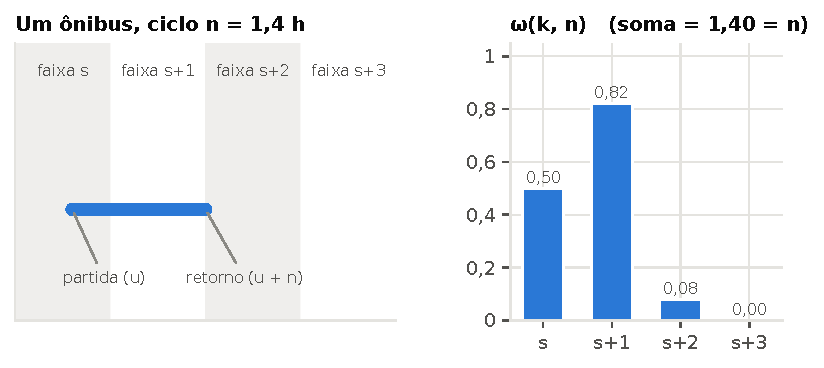
\includegraphics[width=0.85\textwidth]{omega_ilustracao.pdf}
\begin{itemize}\small
\item $\omega(k,n)$: fração da faixa $s+k$ em que um ônibus que partiu em $s$ ainda está rodando
\item $\sum_k \omega(k,n) = n$ $\Rightarrow$ frota = frequência $\times$ ciclo (Ceder, 2016) com frequência constante
\item Captura o \destaque{início do pico}: os ônibus das 6h ainda ocupam a frota às 7h
\end{itemize}
\end{frame}

% ---------------------------------------------------------------- 5
\begin{frame}{Dados e calibração da demanda}
\begin{columns}[T]
\column{0.5\textwidth}
\textbf{Oferta (GTFS da BHTRANS)}
\begin{itemize}\small
\item Ciclos e extensões por linha e hora
\item $F=\frotaMax$: frota que a grade atual exige (cadastro MOVE: \frotaMOVE{}, todos os corredores, com reserva)
\item $\bar P=\capCorredor$ partidas/h: pico programado hoje
\end{itemize}
\column{0.48\textwidth}
\textbf{Demanda (relatórios BHTRANS)}
\begin{itemize}\small
\item Embarques por dia útil; nas estações, a catraca não identifica a linha
\item Rateio $\Rightarrow$ intervalo de \demandaInf{} a \demandaSup{} emb./dia ($\lambda$ de 0 a 1)
\item \destaque{Calibração:} $\lambda=\lambdaCentral$ $\Rightarrow$ grade atual com ocupação média de 100\%
\item Por linha, a grade satura entre $\lambda=\lambdaMinLinha$ e \lambdaMaxLinha{}: efeito do rateio
\end{itemize}
\end{columns}
\vspace{0.3em}
\small Custos, capacidades, padrão de serviço e $\alpha_2$: \destaque{hipóteses} declaradas (tabela no apoio).
\end{frame}

% ---------------------------------------------------------------- 6
\begin{frame}{Solução: Gurobi, branch-and-cut}
\begin{columns}[T]
\column{0.5\textwidth}
\begin{enumerate}\small
\item Presolve
\item Relaxação linear (simplex): R\$~\Zrelax
\item Cortes: \destaque{\cortesGomory{} Gomory, \cortesMIR{} MIR}
\item Heurísticas
\item Branch-and-bound (se necessário)
\end{enumerate}
\column{0.48\textwidth}
\begin{block}{Log do Gurobi \versaoGurobi}
\small Ótimo no nó raiz, \iteracoesSimplex{} iterações, \tempoSolucao\,s, gap final \gapFinal\%.\\[3pt]
Os cortes fecharam o gap de integralidade de \gapInt\%.
\end{block}
\end{columns}
\end{frame}

% ---------------------------------------------------------------- 7
\begin{frame}{Validação: grade atual $\times$ ótimo, no mesmo modo}
\centering
\resizebox{0.95\linewidth}{!}{\begin{tabular}{llrrrrr}
\toprule
Modo & Solução & Viagens & Custo (R\$) & Não atendidos & Indicador & $Z$ (R\$) \\
\midrule
fila & Grade atual (GTFS) & 664 & 242.902 & 50.301 pas$\cdot$h & 34{,}97 min/pas & 1.500.427 \\
fila & Solução ótima & 712 & 264.417 & 465 pas$\cdot$h & 0{,}32 min/pas & 276.042 \\
\midrule
perda & Grade atual (GTFS) & 664 & 242.902 & 4.245 pas & 4{,}92\% perdidos & 349.027 \\
perda & Solução ótima & 708 & 262.994 & 392 pas & 0{,}45\% perdidos & 272.794 \\
\bottomrule
\end{tabular}
}
\vspace{0.6em}
\begin{itemize}\small
\item Ótimo: \destaque{mais serviço por mais custo} (+\variacaoCusto\% de custo, +\variacaoViagens\% de viagens)
\item Total por linha $\approx \sum_t\lceil d/C\rceil$: segue a \destaque{regra de rateio}, não é validação independente
\item O ganho do modelo está na \destaque{distribuição horária} e no acoplamento pela frota
\end{itemize}
\end{frame}

% ---------------------------------------------------------------- 8
\begin{frame}{Resultados dependem da demanda ($\lambda$)}
\centering
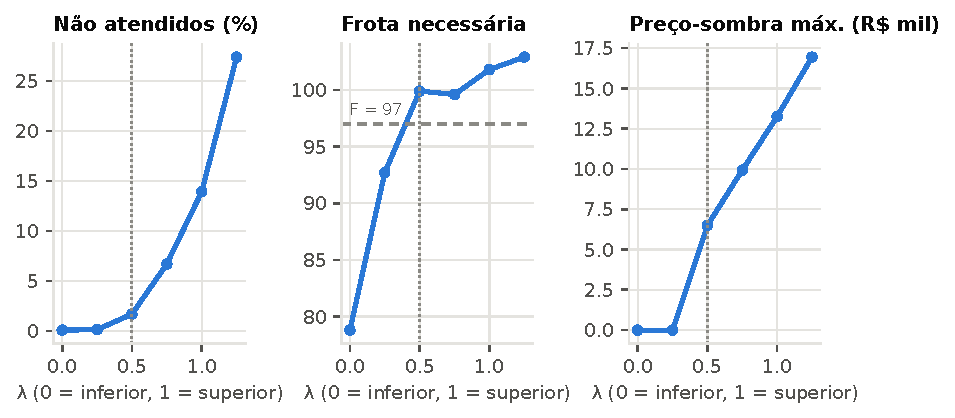
\includegraphics[width=0.88\textwidth]{demanda_lambda.pdf}
\begin{itemize}\small
\item $\lambda=\lambdaCentral$: espera de \esperaMin{} min/pas; frota no limite só às \horaPrecoMax
\item Escassez de frota (preço-sombra $>0$) a partir de $\lambda\approx\lambdaGargalo$; no limite inferior, a frota sobra
\item $\lambda=1$: +10 articulados reduzem a espera de \esperaBaseUm{} para \esperaMaisDezArtUm{} min/pas; corredor +20\%, só para \esperaCorredorUm
\end{itemize}
\end{frame}

% ---------------------------------------------------------------- 9
\begin{frame}{Cenários: o modelo escolhe o tipo de veículo}
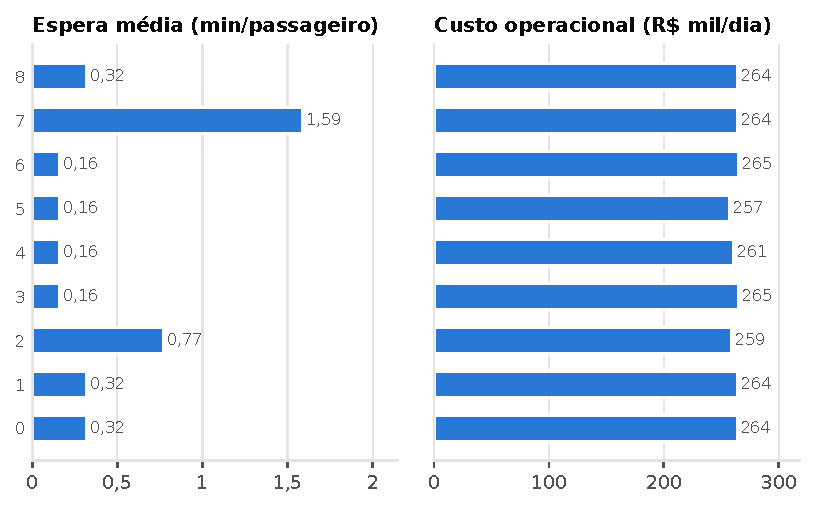
\includegraphics[width=0.58\textwidth]{cenarios.pdf}\hfill
\begin{minipage}[b]{0.39\textwidth}\small
\begin{itemize}
\item 90 articulados: espera sobe para \esperaFnoventa{} min/pas
\item +15 Padron: \esperaPadron{} min/pas e custo operacional menor
\item \destaque{Mas}: sem aquisição e tripulação, e com R\$/km hipotético. Com custo/km igual ao articulado, compensa até R\$~\equilibrioPadronIgual/veíc.$\cdot$dia
\item +10 articulados (mesma capacidade): até R\$~\equilibrioMaisDezArt/veíc.$\cdot$dia
\end{itemize}
\end{minipage}
\end{frame}

% ---------------------------------------------------------------- 10
\begin{frame}{Fronteira de Pareto e o peso $\alpha_2$}
\begin{columns}[c]
\column{0.58\textwidth}
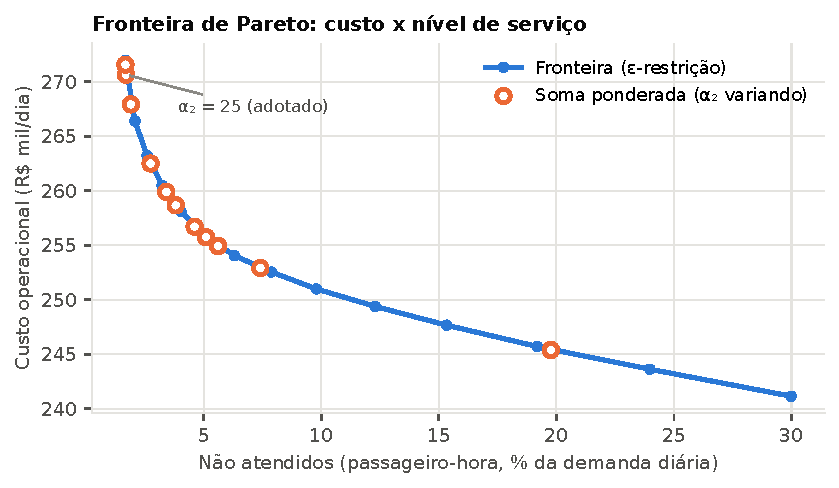
\includegraphics[width=\textwidth]{fronteira_pareto.pdf}
\column{0.4\textwidth}
\small
\begin{itemize}
\item $\varepsilon$-restrição: min custo s.a. espera $\le \varepsilon$
\item Perto do melhor serviço, reduzir 1 passageiro-hora custa cerca de R\$~\custoMarginalPareto
\item Para $\alpha_2$ acima de $\sim$R\$~\custoMarginalPareto, o ganho é marginal $\Rightarrow$ solução \destaque{quase lexicográfica}
\item A fronteira mostra as alternativas
\end{itemize}
\end{columns}
\end{frame}

% ---------------------------------------------------------------- 11
\begin{frame}{Limitações e conclusões}
\begin{columns}[T]
\column{0.48\textwidth}
\textbf{Limitações}
\begin{itemize}\small
\item Demanda = embarques rateados, não carga medida
\item Diferença entre linhas vem do rateio
\item Padron sem custo fixo; custos/km hipotéticos
\end{itemize}
\column{0.48\textwidth}
\textbf{Conclusões}
\begin{itemize}\small
\item PLIM exato em $<1$\,s com frota acumulada, fila, corredor e tipos de veículo
\item Demanda calibrada: mais serviço por +\variacaoCusto\% de custo
\item Escassez de frota no pico da manhã só para $\lambda\gtrsim\lambdaGargalo$
\item Frota extra: articulado rende mais por veículo, salvo se o Padron for bem mais barato
\end{itemize}
\end{columns}
\vspace{1em}
\begin{center}\Large\color{marinho}\textbf{Obrigado! Perguntas?}\end{center}
\end{frame}

% ================================================================ apoio
\appendix

\begin{frame}{Apoio: dualidade -- quanto vale um ônibus a mais?}
\centering\scriptsize
\resizebox{0.9\linewidth}{!}{\begin{tabular}{lrrcr}
\toprule
Faixa & Frota (PL) & Preço-sombra (R\$) & Validade do RHS & $\Delta Z$ PLIM, +1 veíc. (R\$) \\
\midrule
7h & 90{,}0 & 2.416{,}98 & 86{,}6 a 97{,}8 & 2.080{,}10 \\
8h & 90{,}0 & 1.632{,}75 & 87{,}5 a 96{,}8 & 1.590{,}24 \\
16h & 88{,}5 & 0{,}00 & 88{,}5 a $\infty$ & 225{,}19 \\
17h & 90{,}0 & 1.659{,}42 & 89{,}3 a 92{,}1 & 976{,}58 \\
18h & 90{,}0 & 1.973{,}46 & 85{,}9 a 90{,}4 & 1.282{,}59 \\
\bottomrule
\end{tabular}
}
\vspace{0.5em}
\begin{itemize}\small
\item Relaxação linear: preço-sombra só $>0$ onde a restrição está ativa (folgas complementares)
\item +1 veículo sai da faixa de validade do RHS $\Rightarrow$ ganho no PLIM menor que o dual
\item \faixasReotimizadas{} faixas re-otimizadas no PLIM; ganho em \faixasGanhoPLIM
\item Duais de R2 (\nPares{} pares): $=c/C$ (\regimeFolga), $>c/C$ (\regimeLimite), $<c/C$ (\regimeSobra), fila (\regimeFila), sem demanda (\regimeSemDemanda)
\end{itemize}
\end{frame}

\begin{frame}{Apoio: frota e espera por hora (demanda calibrada)}
\centering
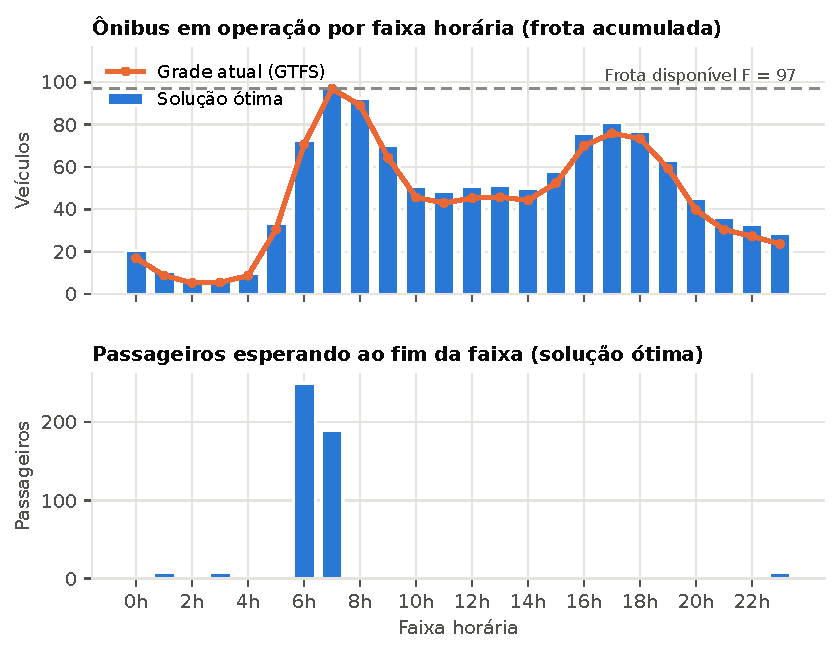
\includegraphics[height=0.8\textheight]{frota_deficit_por_hora.pdf}
\end{frame}

\begin{frame}{Apoio: parâmetros e origem}
\centering
\resizebox{\linewidth}{!}{\begin{tabular}{p{3.4cm}p{8.0cm}p{2.6cm}}
\toprule
Parâmetro & Valor & Origem \\
\midrule
Frota disponível $F$ & 97 articulados em operação (exigidos pela grade atual); a frota cadastrada do BRT MOVE é de 457 veículos em todos os corredores, incluindo reserva técnica & GTFS; BHTRANS \\
Capacidade do corredor $\bar{P}$ & 64 partidas/h (maior valor programado hoje) & GTFS \\
Tempo de ciclo $n_{lt}$ & duração da viagem circular $+15\%$ & GTFS + hipótese \\
Extensão $D_{lt}$ & geometria do itinerário (ida e volta) & GTFS \\
Demanda $d_{lt}$ & embarques/h atribuídos à linha; $\lambda=0{,}435$ (calibrado) & BHTRANS + hipótese de rateio \\
Capacidade $C_k$ & articulado 130; Padron 85 passageiros & Hipótese \\
Custo por km & articulado R\$ 12{,}50; Padron R\$ 9{,}50 & Hipótese \\
$f^{\min}_{lt}$ & intervalo máximo de 10 min no pico ($\ge6$/h), 20 min de dia ($\ge3$/h) e 60 min à noite ($\ge1$/h) & Hipótese \\
$f^{\max}_{lt}$ & 24 partidas/h por linha (intervalo de 2,5 min) & Hipótese \\
$\alpha_1$, $\alpha_2$ & 1; R\$ 25 por passageiro-hora & Hipótese \\
\bottomrule
\end{tabular}
}
\end{frame}

\begin{frame}{Apoio: respostas a perguntas prováveis}
\scriptsize
\begin{itemize}
\item \textbf{Viagens saem da 52 e 63 por quê?} Efeito do rateio: a grade dessas linhas só satura em $\lambda\approx\lambdaMaxLinha$; a da 64, em $\lambda\approx\lambdaMinLinha$.
\item \textbf{Por que este $\lambda$?} Calibrado: a grade que opera hoje teria ocupação média de 100\%.
\item \textbf{Quanto custa a grade atual?} R\$~\custoGTFS/dia, contra R\$~\custoTotal{} do ótimo, que atende mais.
\item \textbf{Padron sem custo de aquisição?} Sim; por isso o custo de equilíbrio por veículo$\cdot$dia e a sensibilidade ao R\$/km.
\item \textbf{Embarque $\times$ carga?} Os dados são embarques; o fator de trecho crítico (= 1) não é identificável separado de $\lambda$.
\item \textbf{Frota necessária não cresce sempre com $\lambda$?} Quando o corredor passa a limitar, parte da espera fica inevitável.
\item \textbf{Por que R\$~\alfaDois/pas$\cdot$h?} Hipótese; acima de $\sim$R\$~\custoMarginalPareto{} o resultado muda pouco (fronteira).
\item \textbf{$w_{l,-1}=0$, mas frota cíclica?} Deliberado: o dia útil começa sem fila; os ônibus da madrugada são poucos.
\end{itemize}
\end{frame}

\begin{frame}{Apoio: demanda ($\lambda$) e robustez}
\centering\scriptsize
\resizebox{\linewidth}{!}{\begin{tabular}{rrrrrrr}
\toprule
$\lambda$ & Demanda/dia & Emb./viagem GTFS & Viagens ótimo & \% não atend. & Frota necessária & Preço-sombra máx. (R\$) \\
\midrule
0{,}00 & 65.266 & 98{,}3 & 571 & 0{,}1 & 78{,}8 & 0 \\
0{,}25 & 77.361 & 116{,}5 & 644 & 0{,}1 & 92{,}7 & 0 \\
0{,}50 & 89.455 & 134{,}7 & 728 & 1{,}7 & 99{,}9 & 6.493 \\
0{,}75 & 101.550 & 152{,}9 & 814 & 6{,}7 & 99{,}6 & 9.928 \\
1{,}00 & 113.645 & 171{,}2 & 907 & 13{,}9 & 101{,}8 & 13.255 \\
1{,}25 & 125.740 & 189{,}4 & 986 & 27{,}4 & 102{,}9 & 16.941 \\
\bottomrule
\end{tabular}
}
\vspace{0.8em}

\resizebox{0.8\linewidth}{!}{\begin{tabular}{lrrrr}
\toprule
Caso & Viagens & Custo (R\$) & Não atendidos & Indicador \\
\midrule
Base (perfil GTFS, fila) & 712 & 264.417 & 465 & 0{,}32 min/pas \\
Perfil horário típico (independente da grade) & 723 & 269.099 & 151 & 0{,}10 min/pas \\
Não atendido desiste (modo perda) & 708 & 262.994 & 392 & 0{,}45 \% perdidos \\
\bottomrule
\end{tabular}
}
\end{frame}

\end{document}
